\begin{figure}[H]
\begin{circuitikz}
\draw
(0,3)to[L](0,2)to[Do](0,1)
(1,3)to[L](1,2)to[Do](1,1)
(2,3)to[L](2,2)to[Do](2,1)
(0,3)to[short](4,3)to[european resistor,l=$Z_\textcyrillic{н}$](4,0.5)
--(1,0.5)--(1,1)
(0,1)--(2,1)
;\end{circuitikz}
\caption{трехфазная нулевая схема}
\end{figure}

ЭДС -- если хотя бы на части периода сохраняет напряжение, то это ЭДС.
1 работник, 2е курят в коридоре. производительность используется на
$\displaystyle \frac{1}{3}$. Если включил активную нагрузку, то получил 
бы $P\sim\frac{1}{3}$ <там среднеквадратичное>.

Если все вентили вывернем, то на нагрузке количественно ничего не изменится
если повернуть 
\begin{circuitikz}\draw
(0,0)to[Do](0,1)
;\end{circuitikz}.
Изменится полярность.

Исторически
\begin{circuitikz}
\draw
(0,1)to[Do](0,0)
(1,1)to[Do](1,0)
(2,1)to[Do](2,0)
(0,0)--(2,0)
;
\draw[thin,<-] (1,0)--(1.8,-0.4) node[right] {жидкий ртутный катод};
\end{circuitikz}
<так и здесь>.

Для сети немного изменится

\begin{circuitikz}
\draw
(0,3)to[short](5,3)
(0,3)to[L](0,2)to[Do,*-](0,1)
(1,3)to[L](1,2)to[Do,*-](1,1)
(2,3)to[L](2,2)to[Do,*-](2,1)

(0,2)--(-0.5,2)--(-0.5,1)
(1,2)--(0.5,2)--(0.5,1)
(2,2)--(1.5,2)--(1.5,1)
(-0.5,0)to[Do,*-](-0.5,1)
(0.5,0)to[Do,*-](0.5,1)
(1.5,0)to[Do,*-](1.5,1)
% нагрузки
(0,1)--(4,1)to[european resistor,l_=$Z_{\textcyrillic{н}'}$](4,3)
(-0.5,0)--(5,0)to[european resistor,l_=$Z_{\textcyrillic{н}''}$](5,3);
\draw[thin,<->](3,1)--(3,3) node[above] {$U_{d'}$};
\draw[thin,<->](6,0)--(6,3) node[right] {$U_{d''}$};
\draw[thin,<-] (5.6,1.2)--(6.7,1) node[right]
{нагрузки $Z_{\textcyrillic{н}'}$ и $Z_{\textcyrillic{н}''}$ одинаковые};
\draw[thin,<-](0.8,0.4)--(1.8,-0.6) node[right]
{Группа ОА --объединенный(общий) анод};
\draw[thin,<-](2.2,1.4)--(3.2,0.4) node[right]
{Группа ОК --объединенный(общий) катод};
\end{circuitikz}

Вентили принадлежат двум группам: Группа ОК и группа ОА.

Прежде был курс ТОЭ --теоретическая часть. Силовая электроника --
практическая часть, будем требовать качественно оформление отчёта.
Продукция -- это техническая документация.

$U_{d'}$ и $U_{d''}$ по величине одинаковые, по фазе отличаются:

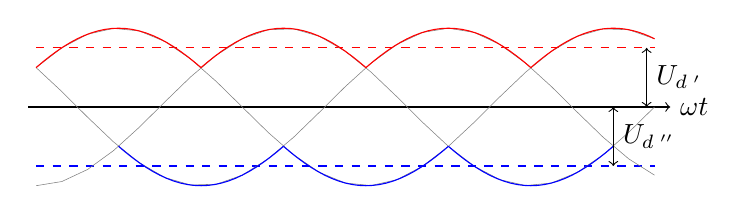
\begin{tikzpicture}
\draw[thin,->] (-pi-0.1,0)--(pi+pi/2+0.2,0) node[right]{$\omega t$};
\draw[thin,dashed,red] (-pi,0.75)--(pi+pi/2,0.75);
\draw[thin,dashed,blue] (-pi,-0.75)--(pi+pi/2,-0.75);
\draw[domain=-pi:pi+pi/2,help lines]
plot(\x, {cos(\x r)})
plot(\x, {cos((\x-2*pi/3) r)})
plot(\x, {cos((\x-4*pi/3) r)});
%u';
\draw[domain=-pi:-pi/3,red]
plot(\x, {cos((\x-4*pi/3) r)});
\draw[domain=-pi/3:pi/3,red]
plot(\x, {cos(\x r)});
\draw[domain=pi/3:pi,red]
plot(\x, {cos((\x-2*pi/3) r)});
\draw[domain=pi:pi+pi/2,red]
plot(\x, {cos((\x-4*pi/3) r)});
%u''
\draw[domain=-2*pi/3:0,blue]
plot(\x, {cos((\x-2*pi/3) r)});
\draw[domain=0:2*pi/3,blue]
plot(\x, {cos((\x-4*pi/3) r)});
\draw[domain=2*pi/3:4*pi/3,blue]
plot(\x, {cos(\x r)});
%
\draw[thin,<->] ({3*pi/2-0.1},0.75)--({3*pi/2-0.1},0)
node[midway,right]{$U_{d\;'}$};
\draw[thin,<->] ({4/3*pi},-0.75)--({4/3*pi},0) 
node[midway,right]{$U_{d\;''}$};
\end{tikzpicture}

Примем допущение, что $L_\Phi$ большая а пульсации маленькие по направлению
не меняются.

Постоянное $\displaystyle \frac{U}{R} =i$ (ток).

В нагрузке сумма $U_\textcyrillic{пост}+U_\textcyrillic{перем}$. Для средних
$u_{d\;'}=u_{d\:''}$.

\underline{Значит токи будут одинаковыми}

Токи одинаковые, но я оторвал: сколько втекает столько вытекает при условии
что переменные пульсации равны. Пульсации равны, но сдвинуты по фазе.

\begin{circuitikz}
  \draw
  (0,3)to[short](6,3)
  (0,3)to[L,*-](0,2)to[Do,*-](0,1)
  (1,3)to[L,*-](1,2)to[Do,*-*](1,1)
  (2,3)to[L,*-](2,2)to[Do,*-*](2,1)
  (0,1)to[short](3,1)to[L,l=$L_\Phi$](4,1)to[short](6,1)
  (4.7,1.4)rectangle(5.3,2.6)
  (5,1)--(5,1.4)
  (5,2.6)--(5,3)
  (4.7,1.4)to[short,v^<=$ $](4.7,2.6)
  (6,1)to[voltmeter](6,3)
  %
  (0,2)--(-0.5,2)--(-0.5,1)
  (1,2)--(0.5,2)--(0.5,1)
  (2,2)--(1.5,2)--(1.5,1)
  (-0.5,0)to[Do,*-](-0.5,1)
  (0.5,0)to[Do,*-](0.5,1)
  (1.5,0)to[Do](1.5,1)
  (1.5,0)to[short](-1.5,0)to[L,l=$L_\Phi$](-2.5,0)
  (-2.8,1.4)rectangle(-2.2,2.6)
  (-2.5,0)to[short](-2.5,1.4)
  (-2.5,2.6)--(-2.5,3)--(0,3)
  (-2.8,1.4)to[short,v^>=$ $](-2.8,2.6)
  (-2.5,1)--(-1.5,1)to[voltmeter](-1.5,3)
  %
  (-1.5,3)to[short,*-](-1.5,3.8)--(5,3.8)to[short,-*](5,3)
  (2,3.3)node{пока не оторвал}
  ;
\draw[thin,red] (3.1,2.9)--(3.2,3.1) 
(3.3,2.9)--(3.4,3.1) (3.5,2.9)--(3.6,3.1) (3.7,2.9)--(3.8,3.1) 
(-1.2,2.9)--(-1.1,3.1) (-1,2.9)--(-0.9,3.1) (-0.8,2.9)--(-0.7,3.1)
(-0.6,2.9)--(-0.5,3.1)
;
\draw[thin,<-] (3.5,0.7) -- (3.8,0.2)node[below]
{$\begin{array}{c}\textcyrillic{допущение, что нет}\\
\textcyrillic{переменной составляющей}\end{array}$};
\draw[thin,<-] (-2.8,1.2)--(-3,-1)node[below]
{$\begin{array}{c}\textcyrillic{последнее, вместо}\\
\textcyrillic{двух нагрузок}\\
\textcyrillic{включаем одну}\end{array}$};
\end{circuitikz}

\subsection{мостовая схема}
Мостовая схема представляет собой последовательное соединение двух 
нулевых схем, одна из которых с ОК, другая с ОА. Но так как
нет соединения с нулём трансформатора, то у трансформатора "0" не
нужен, и вместо звезды у трансформатора может быть треугольник.

Нулевая схема выпрямления предполагает, что все обмотки трансформатора
соединены в m-фазную звезду с выведенным нулём и все концы в звезде
(либо все с точкой, либо все без точки) объединены, а нагрузка включена
между ... При этом на нагрузке напряжение больше

\begin{tikzpicture}
\draw[thin,->] (-2*pi/3-0.1,0)--(2*pi+0.2,0) node[right]{$\omega t$};
%\draw[thin,dashed,red] (-pi,0.75)--(pi+pi/2,0.75);
%\draw[thin,dashed,blue] (-pi,-0.75)--(pi+pi/2,-0.75);
\draw[domain=-2*pi/3:2*pi,help lines]
plot(\x, {cos(\x r)})
plot(\x, {cos((\x-2*pi/3) r)})
plot(\x, {cos((\x-4*pi/3) r)});
\draw[domain=pi/2:3*pi/2,help lines,loosely dashed]
plot(\x, {-cos(\x r)});
\draw[domain=-2*pi/3:pi/6,help lines,loosely dashed]
plot(\x, {-cos((\x-2*pi/3) r)});
\draw[domain=-pi/6:5*pi/6,help lines,loosely dashed]
plot(\x, {-cos((\x-4*pi/3) r)});
%суммы
\draw[domain=0:pi/3]
plot(\x, {cos(\x r) - cos((\x-4*pi/3) r)}); %a - c
\draw[domain=pi/3:2*pi/3]
plot(\x, {cos((\x-2*pi/3) r)- cos((\x-4*pi/3) r)}) ;% b-c
\draw[domain=2*pi/3:pi]
plot(\x, {cos((\x-2*pi/3) r)-cos(\x r)});%b-a
\draw[domain=pi:4*pi/3]
plot(\x, {cos((\x-4*pi/3) r)-cos(\x r)});%c-a
\draw[domain=4*pi/3:5*pi/3]
plot(\x, {cos((\x-4*pi/3) r)-cos((\x-2*pi/3) r)});%c-b
\draw[domain=5*pi/3:2*pi]
plot(\x, {cos(\x r)-cos((\x-2*pi/3) r)});%a-b

\draw (0,1) node[above]{a} 
(2*pi/3,1) node[above]{b}
(4*pi/3,1) node[above]{c}
(-pi/3,-0.5) node{$V_6$}
(0,0.5) node{$V_1$}
(pi/3,-0.5) node{$V_2$}
(2*pi/3,0.5) node{$V_3$}
(pi,-0.5) node{$V_4$}
(4*pi/3,0.5) node{$V_5$}
(5*pi/3,-0.5) node{$V_6$}
(pi/6, {sqrt(3)}) node[rotate=90,right] {$V_1-V_2$}
(pi/6+pi/3, {sqrt(3)}) node[rotate=90,right] {$V_3-V_3$}
(pi/6+2*pi/3, {sqrt(3)}) node[rotate=90,right] {$V_3-V_4$}
(pi/6+pi, {sqrt(3)}) node[rotate=90,right] {$V_5-V_4$}
(pi/6+4*pi/3, {sqrt(3)}) node[rotate=90,right] {$V_5-V_6$}
(pi/6+5*pi/3, {sqrt(3)}) node[rotate=90,right] {$V_1-V_6$}
;

\draw[domain=-pi/3:pi/3,red]
plot(\x, {cos(\x r)});
\draw[domain=pi/3:pi,red]
plot(\x, {cos((\x-2*pi/3) r)});
\draw[domain=pi:5*pi/3,red]
plot(\x, {cos((\x-4*pi/3) r)});
%
\draw[domain=-2*pi/3:0,blue]
plot(\x, {cos((\x-2*pi/3) r)});
\draw[domain=0:2*pi/3,blue]
plot(\x, {cos((\x-4*pi/3) r)});
\draw[domain=2*pi/3:4*pi/3,blue]
plot(\x, {cos(\x r)});
\draw[domain=4*pi/3:2*pi,blue]
plot(\x, {cos((\x-2*pi/3) r)});
%
\draw[thin,<-] (2*pi+0.1, 1.5)--(2*pi+0.9,1.5) node[right] 
{$\textcyrillic{везде }1\frac{1}{2}\textcyrillic{ амплитуды}$};
\draw[thin,<-] (pi/6+5*pi/3+0.2, {sqrt(3)+0.1}) -- (2*pi+0.9,2)
node[right] {$\sqrt{3}$};
\draw (2*pi+0.5, 0.6) node (a) {};
\draw (2*pi+0.7,-1) node {} edge[bend right=45,->]
node[midway,right]{$\begin{array}{c}\textcyrillic{добавить с обратным}\\
\textcyrillic{знаком}\end{array}$}
(a.south);
\end{tikzpicture}

3-х пульсная кривая, <название> некрасивое, но правильное.
Например: 

\begin{tabular}{ccc}
3-х фазная нулевая & - & 3-х пульсная\\
3-х фазная мостовая  & - & 6-ти пульсная
\end{tabular}

Амплитуде пульсаций уменьшилась. 

\begin{circuitikz}
\draw
(5,1)to[Do,l=$V_2$,-*](4,1)--(2,1)to[Do,l=$V_5$](1,1)
(5,2)to[Do,l=$V_6$](4,2)to[short,-*](3,2)--(2,2)to[Do,l=$V_3$](1,2)
(5,1)--(5,3)to[Do,l=$V_4$](4,3)--(2,3)to[Do,l=$V_1$,*-](1,3)--(1,1)
(1,2)--(0.5,2)--(0.5,0)--(2,0)
(5,2)--(5.5,2)--(5.5,0)--(4,0)
(3,0) node {$Z_\textcyrillic{н}$}
(2,3)--(2,4) node[above]{a}
(3,2)--(3,4) node[above]{b}
(4,1)--(4,4) node[above]{c}
;\end{circuitikz}

ГОСТ требует нумеровать столбцами, здесь пронумеровано по смыслу:
вентили проводят в порядке
$V_5-V_6$, $V_1-V_6$, $V_1-V_2$, $V_3-V_2$, $V_3-V_4$, $V_5-V_4$. Это
нужно запомнить.

Уменьшилась амплитуда $\Rightarrow$ улучшились условия подавления пульсаций.

%http://www.artofproblemsolving.com/wiki/index.php/LaTeX:Symbols
\begin{tabular}{ccc}
апплитуда $\nearrow$ & $\Rightarrow$ & L $\searrow$\\
$\omega$ $\nearrow$ & $\Rightarrow$ & L $\searrow$ 
\end{tabular}

Размах <пульсаций нулевой схемы> -- 0.5

Сумма двух синусоид, также синусоида

Размах <пульсаций ... схемы> -- 0.13
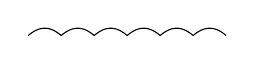
\begin{tikzpicture}\begin{scope}[scale=0.4]
%суммы
\draw[domain=0:pi/3]
plot(\x, {cos(\x r) - cos((\x-4*pi/3) r)}); %a - c
\draw[domain=pi/3:2*pi/3]
plot(\x, {cos((\x-2*pi/3) r)- cos((\x-4*pi/3) r)}) ;% b-c
\draw[domain=2*pi/3:pi]
plot(\x, {cos((\x-2*pi/3) r)-cos(\x r)});%b-a
\draw[domain=pi:4*pi/3]
plot(\x, {cos((\x-4*pi/3) r)-cos(\x r)});%c-a
\draw[domain=4*pi/3:5*pi/3]
plot(\x, {cos((\x-4*pi/3) r)-cos((\x-2*pi/3) r)});%c-b
\draw[domain=5*pi/3:2*pi]
plot(\x, {cos(\x r)-cos((\x-2*pi/3) r)});%a-b
\end{scope}
\end{tikzpicture}

При той же индуктивности ...

3-х фазная схема самая распространенная схема выпрямления.

Достоинства: в 2 раза возрастает частота пульсации. примерно в 2 раза,
почему, потому что мы считали для $\alpha=0$, при $\alpha\ne 0$ будет 
другая форма кривой напряжения. Примерно в два раза возрастет 
продолжительность протекания тока вентильных обмоток. Вентили раборают
$1/6$ периода, обмотки -- $1/3$.Ток течёт по двум обмоткам.
В 2 раза по среднеквадратичному. При том же выпрямленном напряжении
в 2 раза уменьшается напряжение, прикладываемое к вентилям.

К вентилю прикладывается междуфазное линейное напряжение. В худшем
случае прикладывается амплтуда.

Для высоковольтной преоьразовательной техники важно

$\rightleftharpoons$ Преобразуем энергию в $\rightleftharpoons$ 


$330$кВ,$1000$кВ (Экибастуз-центр)

ПУЭ -- правила цстройства электроустановок.

Есть разные категории потребителей. Доменная печь высотой с Исаакиевский собор.
Задули электрическую печь кокс+уголь+флюс. Если электроснабжение прекратилось
чугун стал в ``козел'' -- нужно выбрасывать.

больницы.

8 мостов -- управляемые

один мост закорачивают.

140 вольт.

Мостовые схемы могут быть с роазным числом фаз.

С пульсациями может быть не так. Амплитуда и число пульсаций
уменьшаются если число фаз нечётное.

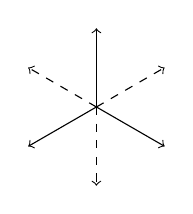
\begin{tikzpicture}
\draw[->](0,0)--(0,1);
\draw[->](0,0)--({cos(90+120)},{sin(90+120)});
\draw[->](0,0)--({cos(90+240)},{sin(90+240)});
\draw[->,dashed](0,0)--({cos(90+60)},{sin(90+60)});
\draw[->,dashed](0,0)--({cos(90+180)},{sin(90+180)});
\draw[->,dashed](0,0)--({cos(90+300)},{sin(90+300)});
\end{tikzpicture}

\begin{tikzpicture}
\begin{scope}[scale=0.7]
\draw[->](0,0)--(0,1);
\draw[thin,dashed] (0,0.5)circle(0.65);
\draw (0.9,0.5) node {+};

\draw[->](0,-0.5)--({cos(90+120)},{sin(90+120)-0.5});
\draw[->](0,-0.5)--({cos(90+240)},{sin(90+240)-0.5});
\draw ({cos(90+240)},{sin(90+240)-0.5}) node[right]{-};

\draw[->](4,0)--(4,1);
\draw[->](4,-0.5)--(4,-1.5);
\draw[thin,<-] (4.2,-0.25)--(5,-1) node[right]
{\begin{tabular}{c}
в чётном числе фаз\\
работают эти
\end{tabular}
};  
\end{scope}
\end{tikzpicture}

\begin{tabular}{ccc}
3-х фазная &--& 6-ти пульсная\\
4-х фазная &--& 4-ти пульсная\\
2-х фазная &--& 2-х <фазная?>
\end{tabular}

Вентили работают 1/6 периода. 
9 обмоток -- вентили работают 1/9, 2/9 периода работают вентильные обмотки.
Рост числа фаз уменьшает коэффициэнт использования вентиля и
трансформатора.

192 фазном выпрямлении эквивалентное

2/3 периода работает обмотка 

Весь период

\begin{tikzpicture}
\draw[thin,->] (-3,0)--(3,0);
\draw (-2,1)--(-0.5,1)--(0.5,-1)--(2,-1);
\draw[dashed] (-0.5,1)--(-0.5,0)--(0.5,0)--(0.5,-1); 
\end{tikzpicture}

Грузится однофазным током

\begin{tikzpicture}
\draw[thin,->] (-3,0)--(3,0);
\draw (-2,1)--(0,1)--(0,-1)--(2,-1);
\end{tikzpicture}

Оптимальное 2.7 между 2 и 3

\begin{tabular}{ccc}
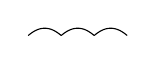
\begin{tikzpicture}\begin{scope}[scale=0.4]
%суммы
\draw[domain=0:pi/3]
plot(\x, {cos(\x r) - cos((\x-4*pi/3) r)}); %a - c
\draw[domain=pi/3:2*pi/3]
plot(\x, {cos((\x-2*pi/3) r)- cos((\x-4*pi/3) r)}) ;% b-c
\draw[domain=2*pi/3:pi]
plot(\x, {cos((\x-2*pi/3) r)-cos(\x r)});%b-a
\end{scope}
\end{tikzpicture}
&
$\Rightarrow$
&
12 пульсов\\
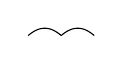
\begin{tikzpicture}\begin{scope}[scale=0.4]
%суммы
\draw[domain=0:pi/3]
plot(\x, {cos(\x r) - cos((\x-4*pi/3) r)}); %a - c
\draw[domain=pi/3:2*pi/3]
plot(\x, {cos((\x-2*pi/3) r)- cos((\x-4*pi/3) r)}) ;% b-c
\end{scope}
\end{tikzpicture}
&
$\Rightarrow$
&
12+12 $\rightarrow$ 24 $\rightarrow$ 48 $\rightarrow$ 96 $\rightarrow$ 192
\end{tabular}

32 моста

Можно последовательно, можно параллельно, параллельно через реактор.

32 ванны (4 параллельных 8 штук)

Кроме улучшения гармонического состава выпрямленного напряжения и тока
повышение числа фаз улучшает гармонический состав
тока потребляемого из сети.

\begin{tikzpicture}
\draw[thin,->] (-pi-0.2,0) -- (pi+0.2,0) node[right]{$\omega t$}; 
\draw[domain=-pi-0.2:pi+0.2]
plot (\x, {-sin(\x r)});
\draw[red] (-pi,0)--(-5*pi/6,0)--(-5*pi/6,{sqrt(3)/2})--
(-pi/6,{sqrt(3)/2})--(-pi/6,0)--(pi/6,0)--(pi/6,{-sqrt(3)/2})--
(5*pi/6,{-sqrt(3)/2})--(5*pi/6,0)--(pi,0);
\draw[thin,<-] (pi/12,{-sin((pi/12) r)}) -- (-0.3,-0.6) node[below]{из сети};
\draw[thin,<-,red] (11*pi/12,0.1)-- (4,0.6) node[right]{разные гармоники}; 
\end{tikzpicture}

Гармоники не 50 Герц, не передают мощности, искажают ток. Это главный 
недостаток выпрямителей.
